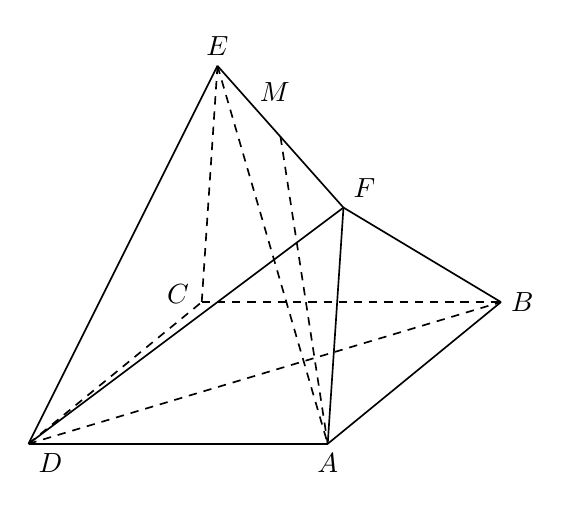
\begin{tikzpicture}[x=1cm,y=1cm,line width=0.6pt]
\coordinate (E) at (3.0000000000,5.4000000000);
\coordinate (F) at (4.6,3.6);
\coordinate (B) at (6.6,2.4);
\coordinate (D) at (0.6,0.6);
\coordinate (A) at (4.4,0.6);
\coordinate (C) at (2.8000000000,2.4000000000);
\coordinate (M) at (3.8000000000,4.5000000000);
% vertical / solid frame
\draw[draw=black,solid] (E) -- (D);
\draw[draw=black,solid] (E) -- (F);
\draw[draw=black,solid] (F) -- (B);
\draw[draw=black,solid] (F) -- (A);
\draw[draw=black,solid] (F) -- (D);
\draw[draw=black,solid] (A) -- (B);
\draw[draw=black,solid] (D) -- (A);
% hidden dashed
\draw[draw=black,dashed,dash pattern=on 3pt off 2.5pt] (E) -- (C);
\draw[draw=black,dashed,dash pattern=on 3pt off 2.5pt] (E) -- (A);

\draw[draw=black,dashed,dash pattern=on 3pt off 2.5pt] (D) -- (C);
\draw[draw=black,dashed,dash pattern=on 3pt off 2.5pt] (D) -- (B);
\draw[draw=black,dashed,dash pattern=on 3pt off 2.5pt] (C) -- (B);
\draw[draw=black,dashed,dash pattern=on 3pt off 2.5pt] (M) -- (A);
% EF midpoint mark: M lies on EF
% labels with clearance
\node[font=\normalsize,anchor=south,xshift=0pt,yshift=0pt] at (E) {$E$};
\node[font=\normalsize,anchor=south west,xshift=0pt,yshift=0pt] at (F) {$F$};
\node[font=\normalsize,anchor=west,xshift=0pt,yshift=0pt] at (B) {$B$};
\node[font=\normalsize,anchor=north west,xshift=0pt,yshift=0pt] at (D) {$D$};
\node[font=\normalsize,anchor=north,xshift=0pt,yshift=0pt] at (A) {$A$};
\node[font=\normalsize,anchor=east,xshift=-1pt,yshift=3pt] at (C) {$C$};
\node[font=\normalsize,anchor=south east,xshift=7pt,yshift=9pt] at (M) {$M$};
\end{tikzpicture}
